% main.tex

\section{Introduction}

The title of this thesis is \emph{Exact Results in $\N=4$ Super Yang-Mills}. A reasonable question to ask is -- why would anyone care about that ? 
After all $\N=4$ is just a toy theory, it is not something that nature implements and thus we can not observe it in particle accelerators, as opposed to say the Standard Model of particle physics. 
And indeed those are all valid points, however there are very good reasons for studying $\N=4$ SYM. 

From a pragmatic point of view, it is the simplest non-trivial quantum field theory in four spacetime dimensions and since attempts at solving realistic QFTs such as the theory of strong interactions (QCD) have so far been futile, it seems like a good starting point -- some go as far as calling it the harmonic oscillator of QFTs. 

Another (and probably the main) reason why $\N=4$ has been receiving so much attention in the last decades is the long list of mysterious and intriguing properties it seems to posses, making it almost an intelectual pursuit of understanding it. 
The theory has been surprising the theoretical physics community from the very beginning: it is a rare instance of a conformal theory in dimensions higher than two, it has a dual description in terms of a string theory and more recently it was discovered to be integrable. 
All of these properties give reasonable hope for actually solving the theory exactly, something that has never been achieved before for any four dimensional interacting QFT.

In the remainder of the section we give a proper introduction to the subject from a historic point of view focusing on its integrability aspect, for it is integrability that allows one to actually find exact results in the theory. We then give an overview of the thesis itself, emphasizing which parts of the text that are reviews of known material and which parts constitute original work.

\subsection{Brief history of the subject}

Quantum field theory has been at the spot light of theoretical physics since the beginning of the century when it was found that electromagnetism is described by the theory of quantum electrodynamics (QED). Since then people have been trying to fit other forces of nature into the QFT framework. 
Ultimately it worked: the theory of strong interactions, quantum chromodynamics or QCD for short, together with the electroweak theory, spontaneously broken down to QED, collectively make up the \emph{Standard Model} of particle physics, which has been extensively tested in particle accelerators since then. 

However nature did not give away her secrets without a fight. 
For some time it was though that strong interactions were described by a theory of vibrating strings, as it seemed to incorporate the so-called Regge trajectories observed in experiments \cite{Veneziano:1968}. 
Even after discovering QCD as a Yang-Mills gauge theory, stringy aspects of it were still evident and largely mysterious. 
Most notably lattice gauge theory calculations at strong coupling suggested that surfaces of color-electric fluxes between quarks could be given the interpretation of stretched strings \cite{Wilson:1974}, thus an idea of a gauge-string duality was starting to emerge. 
It was strongly re-enforced by t'Hooft, who showed that the perturbative expansion of $U(N)$ gauge theories in the large $N$ limit could be rearranged into a genus expansion of surfaces triangulated by the Feynman diagrams, which strongly resembles string theory genus expansions \cite{THooft:1974}.

\vspace{20pt}
\newlength\yearposx
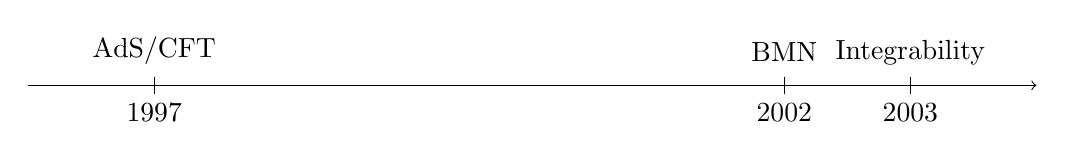
\begin{tikzpicture}[scale=1.6]

    \foreach \x in {1996,1997,2002,2003,2004}{
        \pgfmathsetlength\yearposx{(\x-1996)*1cm};
        \coordinate (y\x)   at (\yearposx,0);
        \coordinate (y\x t) at (\yearposx,+2pt);
        \coordinate (y\x b) at (\yearposx,-2pt);
    }
	
    \draw [->] (y1996) -- (y2004);
    \foreach \x in {1997,2002,2003} \draw (y\x t) -- (y\x b);

	\node at (y1997) [below=3pt] {1997}; \node at (y1997) [above=4pt] {AdS/CFT}; 
	\node at (y2002) [below=3pt] {2002}; \node at (y2002) [above=5pt] {BMN}; 
	\node at (y2003) [below=3pt] {2003}; \node at (y2003) [above=4pt] {Integrability}; 
\end{tikzpicture}
\vspace{20pt}

However it was the work of Maldacena in 1997 that sparked a true revolution \cite{Maldacena:1997re}. He formulated the first concrete conjecture for a duality between a gauge theory, the maximally supersymmetric $\N=4$ super Yang-Mills, and type IIB string theory on $\adsfive$, now universally referred to as the AdS/CFT duality.

\vspace{20pt}
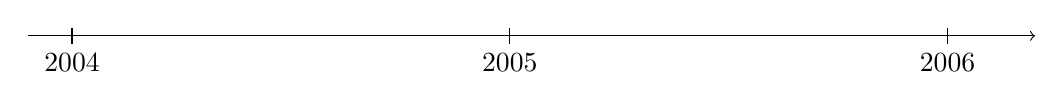
\begin{tikzpicture}[scale=5.56]
    
	\coordinate (start) at (0,0);
	\coordinate (end) at (2.3cm,0);
	
    \foreach \x in {2004,2005,2006}{
        \pgfmathsetlength\yearposx{((\x-2004)*1cm + 0.1cm)};
        \coordinate (y\x)   at (\yearposx,0);
        \coordinate (y\x t) at (\yearposx,+0.5pt);
        \coordinate (y\x b) at (\yearposx,-0.5pt);
    }
	
    \draw [->] (start) -- (end);
    \foreach \x in {2004,2005,2006} \draw (y\x t) -- (y\x b);

	 \node at (y2004) [below=3pt] {2004}; 
		% \node at (y2003) [above=4pt] {AdS/CFT}; 
	 \node at (y2005) [below=3pt] {2005}; 
		% \node at (y2004) [above=5pt] {KMMZ}; 
	 \node at (y2006) [below=3pt] {2006}; 
		% \node at (y2006) [above=4pt] {ABA}; 
\end{tikzpicture}
\vspace{20pt}

Very rapid development.

\vspace{20pt}
\begin{tikzpicture}[scale=1.28]

	\coordinate (start) at (0,0);
	\coordinate (end) at (6.5cm,0);
	
    \foreach \x in {2008,2009,2010,2012,2014}{
        \pgfmathsetlength\yearposx{(\x-2008)*1cm + 0.4cm};
        \coordinate (y\x)   at (\yearposx,0);
        \coordinate (y\x t) at (\yearposx,+2pt);
        \coordinate (y\x b) at (\yearposx,-2pt);
    }
    
    \draw [-] (0,0) -- (7cm,0);
    \draw [decorate, decoration={snake, segment length=5mm, amplitude=1mm}] (7cm,0) -- (8.05cm,0);
	\draw [->] (8.05cm,0) -- (10cm,0);
	
	% draw ticks
	\foreach \x in {2008,2009,2010,2014}
        \draw (y\x t) -- (y\x b);
		
	\draw (8.9cm,-2pt) -- (8.9cm,+2pt);
	\node at (8.9cm,0) [below=4pt] {??}; \node at (8.9cm,0) [above=8pt] {$\N=4$ solved!}; 
	
	%\node at (y1997) [below=3pt] {1997}; \node at (y1997) [above=4pt] {AdS/CFT}; 
	%\node at (y2002) [below=3pt] {2002}; \node at (y2002) [above=5pt] {BMN}; 
	%\node at (y2003) [below=3pt] {???}; \node at (y2003) [above=4pt] {$\N=4$ solved!}; 
\end{tikzpicture}
\vspace{20pt}

Exact solutions. Bright future ahead.

\subsection{Thesis overview}

Maybe a nice picture for the structure of the thesis.
